% !TeX program = lualatex

\documentclass[12pt]{report}
\usepackage[Glenn]{fncychap}
\usepackage[T1]{fontenc}
\usepackage[francais]{babel}
\usepackage{fontspec}
\usepackage{wrapfig}
\usepackage{graphicx}
\usepackage{subcaption}
\usepackage{caption}
\usepackage{soul}
\usepackage[colorlinks=true, linkcolor=black, urlcolor=black, citecolor=black]{hyperref}
% \usepackage[hyphens, spaces, obeyspaces]{url}
\usepackage[a4paper, width=175mm, top=25mm, bottom=25mm]{geometry}
\usepackage{parskip}
\usepackage{enumitem}
\usepackage{titlesec}
\usepackage{listings}
\usepackage{float}
\usepackage[final]{pdfpages}
\usepackage{xcolor}
\usepackage{tocbibind}
\usepackage{tocloft}
\usepackage{xpatch}
\usepackage{amsmath}
\usepackage{amsthm}
\usepackage{amsfonts}
\usepackage{graphics}
\usepackage{color}
% \usepackage[grey,utopia]{quotchap}
\usepackage{moreverb}
\usepackage{xcolor}
\usepackage{framed}
%\usepackage{arabluatex}
\usepackage[ruled,french,onelanguage]{algorithm2e}
\setlist[itemize]{label=\textbullet}
\usepackage{fancyhdr}
\pagestyle{fancy}   
\fancyhead{}
\fancyhead[C]{\leftmark}
\renewcommand{\headrulewidth}{0.4pt}
\renewcommand{\footrulewidth}{0.4pt}
\usepackage{xcolor}
\definecolor{light-gray}{gray}{0.90}
\usepackage{multirow}
\usepackage{soul}
\usepackage[utf8x]{inputenc}
\setcounter{secnumdepth}{3} 
\usepackage{dirtytalk}
\usepackage{csquotes}
\usepackage{mathtools}
\usepackage{amsmath}
\begin{document}

\includepdf[pages=1]{Page_garde.pdf} 
\tableofcontents
\listoffigures
\listoftables


\pagenumbering{arabic}
\newpage

\setlist[itemize]{label=\textbullet}
\chapter{Introduction}
	\section{Problématique et objectifs }
	\paragraph{}
	Dans le domaine de la résolution de problèmes, nous faisons souvent appel à des 
	techniques et algorithmes dits \textbf{intelligents} pour la recherche d'éventuelles
	solutions. Les problèmes de satisfaction de contraintes en sont un exemple, ainsi le
	paradigme de la  programmation par contraintes à été introduit pour modéliser ces 
	et résoudre ces types de problèmes, en introduisant des méthodes venant de la théorie
	des ensembles et de la logique mathématique.
	\par 
	Dans ce projet, nous allons proposer notre propre implémentation d'une version d'un 
	algorithme bien connu de résolution d'un PSC\footnote{Problème de Satisfaction de Contraintes}
	, à savoir l'algorithme \textbf{Look-Ahead} avec filtrage \textbf{PC1 }et \textbf{PC2}.
	\par 
	Avant de commencer nous devons tout d'abord définir dans ce chapitre quelques notions
	théoriques(section suivante), puis présenter le squelette des algorithmes utilisés,
	puis nous définirons dans le chapitre suivant les principales composantes de notre
	système, nous finirons ensuite par une comparaison entre les deux types de filtrage
	utilisés sur deux PSC, l'un connu et un autre dont les paramètres sont générés 
	aléatoirement. Nous conclurons ce travail par une conclusion générale récapitulant 
	l'ensemble des connaissances apprises.

	\section{Définitions}
	\paragraph{}
	Dans cette section nous allons définir les composantes théoriques d'un PSC, ainsi que 
	ceux d'un algorithme de résolution d'un PSC.
	
	\subsection{Problème de Satisfaction de Contraintes}
	\paragraph{}
	Un PSC, est formellement définie comme étant un triplet $<X,D,C>$, où : 
	\begin{itemize}
		\item $X = \lbrace x_1,x_2,...,x_n\rbrace$ est l'ensemble des variables du PSC.
		\item $D = \lbrace D_1,D_2,...,D_n\rbrace$  est l'ensemble des domaines des variables, c'est-à-dire que pour tout $k\in [1;n]$ nous avons $x_k \in D_k$.
		\item $C = \lbrace C_1,C_2,...,C_m\rbrace$ est un ensemble de contraintes. Une contrainte $C_i = (X_i,R_i)$ est définie par l'ensemble $X = \lbrace x_{i_1},x_{i_2},...,x_{i_n} \rbrace$ des variables sur lequel elle porte et la relation $R \subset D_{i_1} \times ... \times D_{i_k}$ qui définit l'ensemble des valeurs que peuvent prendre simultanément les variables de $X_i$
	\end{itemize}
	
	\subsection{Consistance d'un PSC}
	\paragraph{}
	Un PSC est dit consistant si l'on parvient à trouver une instanciation des variables $X_i$ tel que toutes les 
	contraintes $C_j$ soient satisfaites en même temps.
	\par 
	Pour ce faire nous utiliserons des algorithmes de recherche de solutions dit intelligents, parmi eux l'algorithme
	\textbf{Look-Ahead}, l'idée est d'instancier des variables une à une en essayant d'appliquer un filtrage des domaines des
	variables non encore instanciées, ainsi, ç l'instanciation d'une variable, le choix de sa valeur sera idéalement 
	plus restreint, et de ce fait le temps de recherche et de détection d'inconsistance sera plus court.
	\par 
	Look-ahead applique au niveau de chaque noeud un filtrage de consistance de chemin\footnote{\url{https://en.wikipedia.org/wiki/Local_consistency}}. Nous allons voir deux algorithme de consistance 
	de chemin, PC1 et PC2.
	\paragraph{Remarque}: 
	Pour les détails théorique, il faut se référer au support de cours qui donne de très bonnes explications. Dans ce rapport
	nous ne présenterons que les algorithmes des différentes méthodes
	
	\paragraph{PC1}
	Nous devons d'abord définir une fonction \textbf{REVISE\_PC}: \\
	
	\begin{algorithm}[H]
		\caption{REVISE\_PC}
		\SetKwInOut{Input}{Entrée}\SetKwInOut{Output}{Sortie}
		\SetKwFunction{gen}{GenererCandidats}
		
		\Input{$(X_i,X_k,X_j ),(X,D,C)$}
		\Output{$VRAI/FAUX$}
		
		
		\Begin
		{
			$temp \gets M_P[i,j]\bigcap M_P[i,k]°MP[k,k]°MP[k,j]$\;
			\eIf{ $temp \neq M_P[i,j]$}
			{
				$M_P[i,j] \gets temp$
				\KwRet{$VRAI$}
				
			}
			{
					\KwRet{$FAUX$}
			}
			
		}
	\end{algorithm}
	
	\par 
	L'algorithme PC1 est le suivant : 
	
	\begin{algorithm}[H]
		\caption{PC1}
		\SetKwInOut{Input}{Entrée}\SetKwInOut{Output}{Sortie}
		\SetKwFunction{gen}{GenererCandidats}
		\SetKwFunction{rev}{REVISE\_PC}
		
		\Input{$(X,D,C)$}
		\Output{$(X,D,C)$}
		
		$Q \gets {(X_i,X_k,X_j)\in X^3 : \lnot (X_i=X_k=X_j)}$\;
		\Repeat{$R = FAUX$}
		{
			$R \gets FAUX$\;
			\ForEach{$(X_i,X_k,X_j)\in Q$}
			{
				\If{\rev{$(X_i,X_k,X_j),(X,D,C) = VRAI$}}
				{
					$R \gets VRAI$\;	
				}
			}
		}
		\KwRet{$(X,D,C)$}\;
	\end{algorithm}
	
		
	\par 
	L'algorithme PC2 est le suivant : 
	
		\begin{algorithm}[H]
		\caption{PC2}
		\SetKwInOut{Input}{Entrée}\SetKwInOut{Output}{Sortie}
		\SetKwFunction{gen}{GenererCandidats}
		\SetKwFunction{rev}{REVISE\_PC}
		
		\Input{$(X,D,C)$}
		\Output{$(X,D,C)$}
		
		$Q \gets {(X_i,X_j) \in X^2 : (i \leq j) \text{ et il existe une contrainte entre } X_i \text{ et } X_j}$\;
		
		\While{$Q \neq \emptyset $}
		{
			$\text{Prendre une paire } (X_i,X_j) \text{ de variables de } Q\text{, et l’en supprimer }: Q \gets Q - \lbrace(X_i,X_j)\rbrace$\;
		}
		
		\For{$k=1$\KwTo $n \land \lnot (k=i=j)$ }
		{
			$temp \gets M_P[i,k] \bigcap M_P[i,j]°M_P[j,j]°M_P[j,k]$\;
			\If{$temp \neq M_P[i,k]$}
			{
				$M_P[i,k] \gets temp$\;
				$M_P[k,i] \gets (temp)^T$\;
				\eIf{$i\leq k$}
				{$ Q\gets Q \bigcup \lbrace(X_i,X_k)\rbrace $\;}
				{$ Q\gets Q \bigcup \lbrace(X_k,X_i)\rbrace $\;}
			}
		
			$temp \gets M_P[k,j] \bigcap M_P[k,i]°M_P[i,i]°M_P[i,j]$\;
			\If{$temp \neq M_P[k,j]$}
			{
				$M_P[k,j] \gets temp$\;
				$M_P[j,k] \gets (temp)^T$\;
				
				\eIf{$k\leq j$}
				{$ Q\gets Q \bigcup \lbrace(X_k,X_j)\rbrace $\;}
				{$ Q\gets Q \bigcup \lbrace(X_j,X_k)\rbrace $\;}
			}
		}
		
		
		\KwRet{$(X,D,C)$}\;
	\end{algorithm}

	\par 
	Enfin l'algorithme look-ahead avec un choix de filtrage : \\
	\begin{algorithm}[H]
		\caption{LOOK-AHEAD}
		\SetKwInOut{Input}{Entrée}\SetKwInOut{Output}{Sortie}
		\SetKwFunction{gen}{GenererCandidats}
		\SetKwFunction{pc}{PC1}
		\SetKwFunction{pcc}{PC2}
		
		
		\Input{$A,(X,D,C)$}
		\Output{$VRAI/FAUX$}
		
		$Consistance \gets $ \pc{$(X,D,C)$} OU $Consistance \gets $  \pcc{$(X,D,C)$}\; 
		
		\If{$\lnot Consistance$}
		{
			\KwRet{$FAUX$}\;
		}
	
		\eIf{ toutes les variables de $X$ sont instanciées}
		{
			\KwRet{$VRAI$}\;
		}
		{
			 $Xi \gets $ variable de $X$ qui n’est pas encore instanciée\;
			 	
			 \For{$ V_i \in D(X_i) $}
			 {
			 	$D\prime (X_i)=\lbrace Vi \rbrace$\;
			 	$D\prime \gets (D - \lbrace D(X_i) \rbrace )\bigcup {D\prime (X_i)}$\;
			 	\If{$Look-Ahead(A \bigcup \lbrace (X_i,V_i)\rbrace,(X,D\prime,C))$}
			 	{
			 		\KwRet{$VRAI$}\;
		 		}
			 }
		 \KwRet{$FAUX$}\;
			
		}
	\end{algorithm}
	
	
	
\chapter{Solution proposées et implémentation}
Dans ce chapitre nous allons voir l'implémentation de l'algorithme lookAhead avec filtrage PC2 tel que décrit dans le chapitre précédent.
\section{Outils utilisés}
Pour l’implémentation de LookAhead nous avons opté à utiliser le langage de programmation C++ qui à la fois garde la rapidité du C tout en donnant la possibilité de modélisation orienté objet, et ceci en utilisant l'IDE de JetBrains CLion.
\begin{figure}[H]
	\centering
	\begin{subfigure}{.5\textwidth}
		\centering
		
\includegraphics[scale=0.3]{imgs/Clion.jpg}
		\label{fig:sub1}
	\end{subfigure}%
	\begin{subfigure}{.5\textwidth}
		\centering
		
\includegraphics[scale=0.08]{imgs/C++.png}
		\label{fig:sub2}
	\end{subfigure}
	\label{fig:test}
\end{figure}
\section{Implémentation}
Notre implémentation de LookAhead avec filtrage PC2 se compose de trois classes principales: Domains, Constraint et Solver.
\subsection{Domains}
Cette classe permet de gérer les domaines des variables, elle contient pour chaque variable son domaine initiale et son domaine courant, c’est à dire après application des algorithmes de filtrage ou instanciation de la variable. Les domaines sont représentés sous forme de listes d'entier.
\subsection{Constraint}
Chaque contrainte C(Xi,Xj) est représentée par une instance de cette classe, cette dernière contient une matrice nxm où n et m sont les tailles des domaines des variables Xi et Xj respectivement. Cette classe facilite les opérations sur les contraintes notamment la transposition, la composition et l’intersection.
\begin{figure}[H]
	\centering
	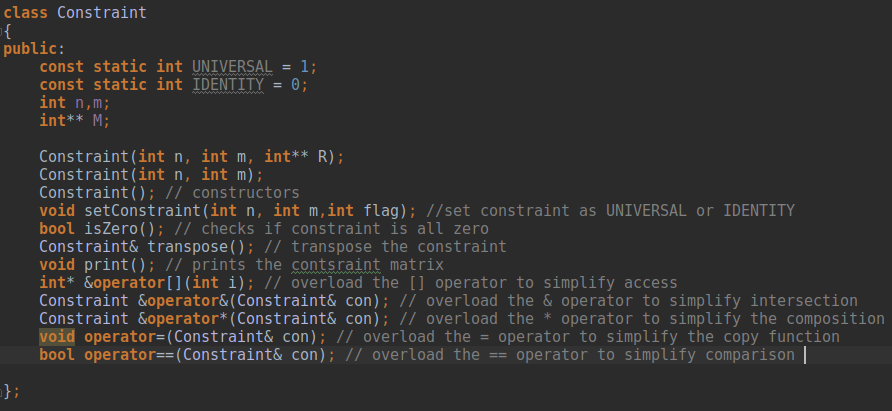
\includegraphics[scale=0.55]{imgs/constraint.png}
	\caption{L'espace de dessin}
	\label{fig:Cons}
\end{figure}
\subsection{Solver}
Un CSP est représenté par cette classe. Elle contient donc les paramètres composant un CSP <X,D,C>: les variables, leurs domaines ainsi que les contraintes entre eux. \\
Nous avons implémenté dans cette classe les algorithmes PC1, PC2 et lookAhead ainsi que la possibilité de choisir la variable à instancier en tirage aléatoire ou en suivant une heuristique.
\paragraph{LookAhead}
L’algorithme lookAhead a été implémenté comme décrit dans la figure \ref{fig:LookAhead}:
\begin{itemize}
\item On applique un filtre et on teste s’il y une inconsistance, sinon si toute les variables ont été instanciées.

\item On choisit la prochaine variable à instancier soit suivant une heuristique ou un ordre aléatoire.

\item On instancie la variable avec les valeurs possibles dans le domaine (qui a été mis à jour par le filtre).

\item On ajoute dans la queue le couple (i,i) pour le prochain appel de PC2.
\end{itemize}
\begin{figure}[H]
	\centering
	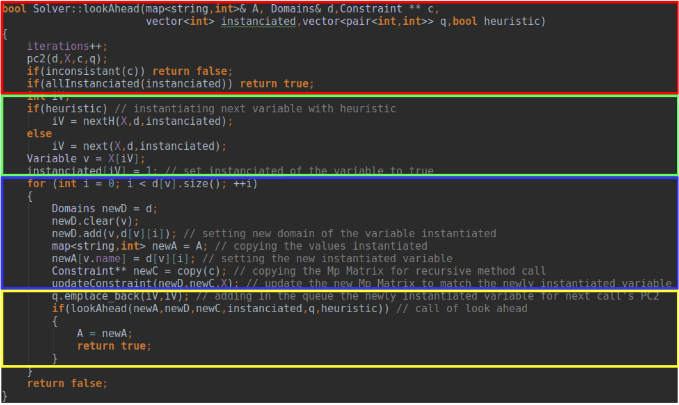
\includegraphics[scale=0.7]{imgs/lookA.png}
	\caption{L'algorithme lookAhead}
	\label{fig:LookAhead}
\end{figure}
\paragraph{Filtrage}
Nous avons implémenté les deux algorithmes de filtrage par chemin PC2 et PC1:
\begin{itemize}
	\item PC1 passe par toutes les variables à chaque fois et applique revise, si une entrée de la matrice Mp change, on refait la même chose.
	\begin{figure}[H]
		\centering
		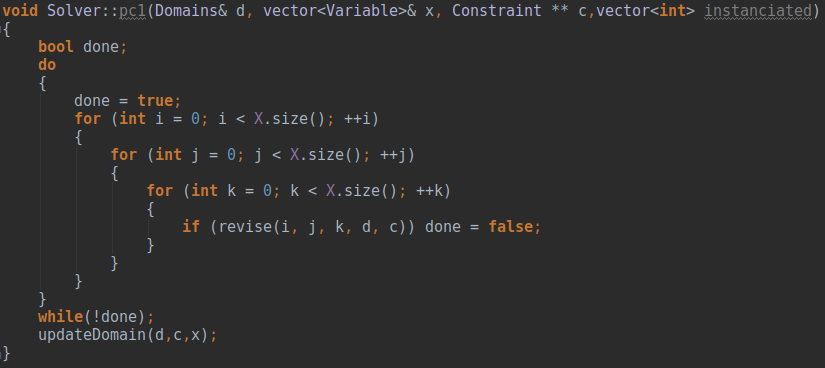
\includegraphics[scale=0.55]{imgs/pc1.png}
		\caption{L'algorithme PC1}
		\label{fig:PC1}
	\end{figure}
	\begin{figure}[H]
		\centering
		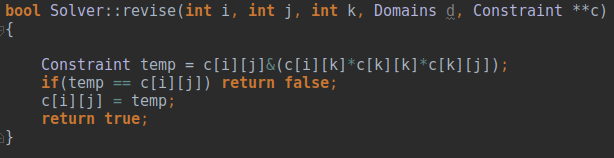
\includegraphics[scale=0.7]{imgs/revise.png}
		\caption{La fonction revise de PC1}
		\label{fig:Revise}
	\end{figure}
	\item PC2 quant à lui utilise une file pour garder les variables dont les entrées de la matrice Mp ont changé afin qu’il les traite.
	\begin{figure}[H]
		\centering
		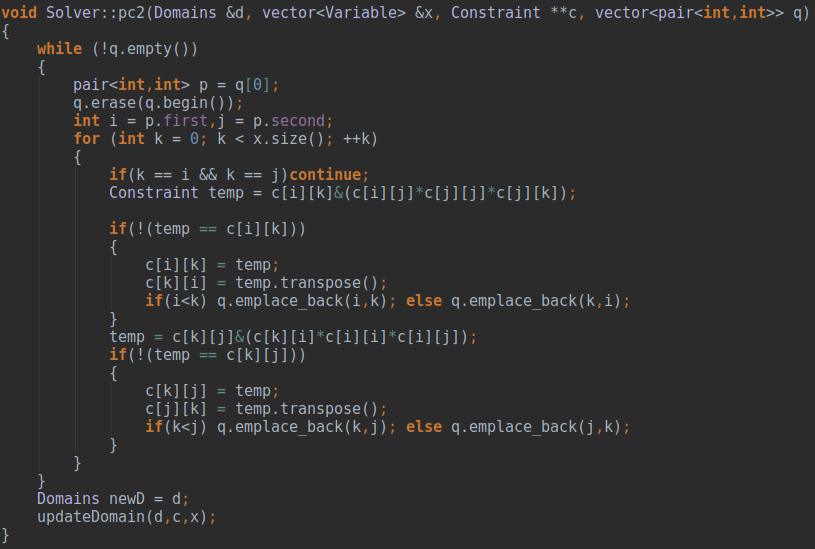
\includegraphics[scale=0.55]{imgs/pc2.png}
		\caption{L'algorithme PC2}
		\label{fig:PC2}
	\end{figure}
\end{itemize}
\paragraph{remarque:}
la fonction \textbf{updateDomain} mis à jour les domains de variables, dans les structures de listes cités avant dans ce chapitre.
\subsection{Génération aléatoire de CSP}
Afin de comparé les deux filtres PC1 et PC2 ainsi que le choix de variables aléatoire ou avec heuristique, nous avons implémenté une fonction qui génère un CSP aléatoire selon les paramètres suivant:
\begin{itemize}
	\item Nombre de variables: c’est le nombre de variables du CSP.
	
	\item Taille du domaine tailleD: la taille des domaines des variables varie entre tailleD*0,5 et tailleD*1,5 aléatoirement.
	
	\item Difficulté: ce paramètre représente la probabilité d’avoir un 0 dans la matrice d’une contrainte du CSP à générer. Plus ce paramètre est élevé, plus le CSP est difficile à satisfaire. 
\end{itemize}

\begin{figure}[H]
	\centering
	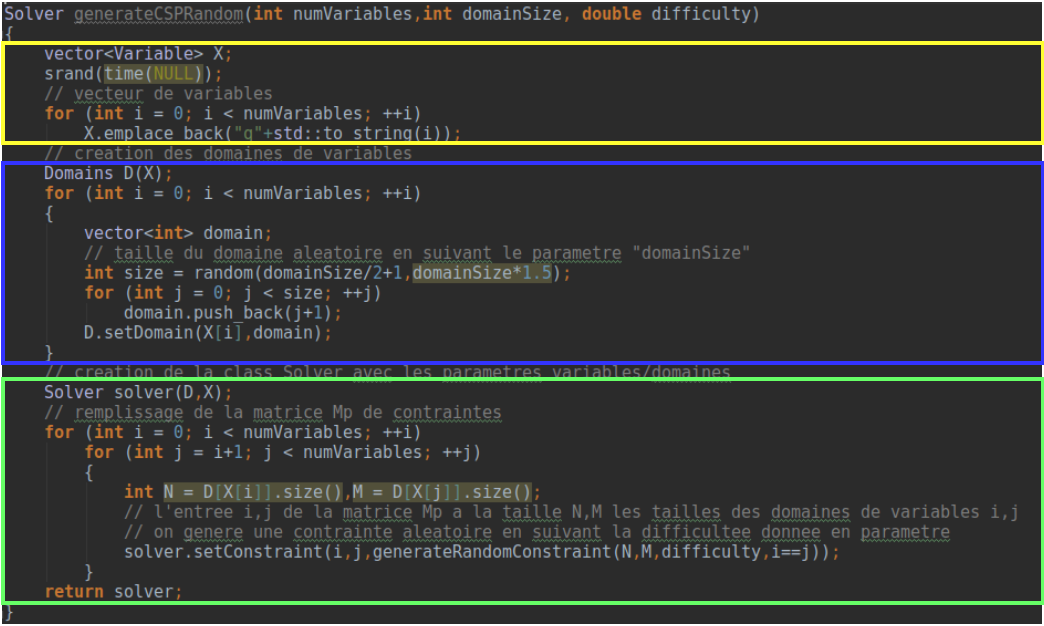
\includegraphics[scale=0.5]{imgs/random.png}
	\caption{L'algorithme PC2}
	\label{fig:Random}
\end{figure}

\section{Résultats}
Nous avons essayé l’algorithme lookAhead d’abord sur un problème connu, le problème des N-Reines. Ensuite nous avons généré des CSP aléatoirement avec des difficultés variables pour tester l’algorithme.
\subsection{N-Reines}
Pour tester les deux filtres PC1 et PC2 avec et sans heuristiques, nous avons généré le problème de N-Reines pour $N \in [4-14]$. les résultats sont résumé dans les figures suivantes:
\begin{figure}[H]
	\centering
	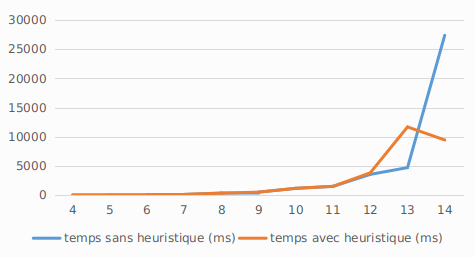
\includegraphics[scale=0.5]{imgs/queen1.png}
	\caption{Résultats de l'application de PC1 sur le problème des N-Reines }
	\label{fig:QueenPC1}
\end{figure}
\begin{figure}[H]
	\centering
	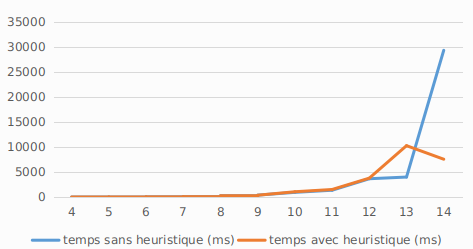
\includegraphics[scale=0.5]{imgs/queen2.png}
	\caption{Résultats de l'application de PC2 sur le problème des N-Reines}
	\label{fig:QueenPC2}
\end{figure}
\paragraph{}
On remarque que dans les deux cas l'heuristique ne donne pas toujours de meilleurs résultats. On remarque aussi que PC2 généralement surpasse PC1 comme le montre les tableaux suivants (les valeurs en rouge sont les valeurs ou PC1 a surpassé PC2):
\begin{figure}[H]
	\begin{tabular}{|c|c|c|c|c|c|c|c|c|c|c|c|}
		\hline
		
		nombre de reines&4&5&6&7&8&9&10&11&12&13&14 \\ \hline
		temps sans heuristique (ms)&2&8&48&85&269&382&937&1359&{\color{red}3659}&3999&{\color{red}29357}\\ \hline
		temps avec heuristique (ms)&3&8&35&71&258&362&1056&{\color{red}1507}&3779&10277&7567\\
		\hline
		
	\end{tabular}%
\caption{temps d'exécution de PC2 par nombre de reines}
\end{figure}
\begin{figure}[H]
	\begin{tabular}{|c|c|c|c|c|c|c|c|c|c|c|c|}
		\hline
		
		nombre de reines&4&5&6&7&8&9&10&11&12&13&14 \\ \hline
		temps sans heuristique (ms)&6&18&57&97&341&506&1143&1486&3542&4703&27391\\ \hline
		temps avec heuristique (ms)&5&17&62&112&317&493&1159&1492&3816&11680&9446\\
		\hline
		
	\end{tabular}%
	\caption{temps d'exécution de PC1 par nombre de reines}
\end{figure}

\subsection{Génération aléatoire de CSP}
Comme nous l’avons vu dans la partie précédente, l’algorithme de génération aléatoire de CSP dépend de trois valeurs: la difficulté, le nombre de variable et le domaine des variables. Dans cette partie nous allons voir comment la variation de un de ces paramètre affecte elle le temps d’exécution de l’algorithme lookAhead avec filtrage PC2.
\paragraph{Difficulté}
La difficulté représente la probabilité d’avoir un 0, donc si cette probabilité est très faible on arrive à satisfaire le CSP rapidement, même chose si elle est très élevé le filtrage PC2 trouve l’inconsistance rapidement. La figure suivante montre l'exécution de l'algorithme en prenant en paramètre le nombre de variable à 10 et le domaine qui varie de 9 à 27, la difficulté quant à elle est dans une échelle de 0 à 20 où la probabilité d’avoir 0 égale à 1 quand la difficulté est égale à 20.
\begin{figure}[H]
	\centering
	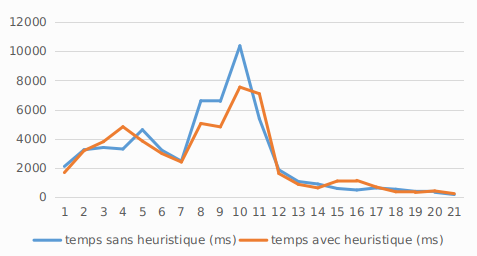
\includegraphics[scale=0.5]{imgs/random2.png}
	\caption{Variation du temps d'exécution selon la difficulté}
	\label{fig:diff}
\end{figure}
\paragraph{Nombre de variables}
Plus on a un nombre de variable est grand, plus le temps de calcule augmente. Dans la figure suivante la difficulté a été fixée à 0,5 tandis que les tailles des domaines de variables varient entre 8 et 22.
\begin{figure}[H]
	\centering
	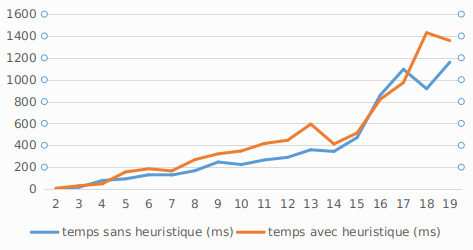
\includegraphics[scale=0.5]{imgs/variables.png}
	\caption{Variation du temps d'exécution selon le nombre de variables}
	\label{fig:vars}
\end{figure}
\paragraph{Taille du domaine}
La taille du domaine est elle aussi relié proportionnellement  au temps d’exécution. Dans la figure suivante la difficulté a été fixée à 0,5 tandis que le nombre de variables varient est à 8.
\begin{figure}[H]
	\centering
	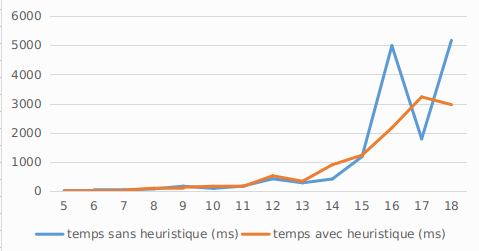
\includegraphics[scale=0.5]{imgs/domain.png}
	\caption{Variation du temps d'exécution selon les tailles des domaines}
	\label{fig:doms}
\end{figure}
\chapter{Conclusion générale}
\paragraph{}
Au terme de projet nous pouvons donc tirer les conclusions suivantes :
\begin{itemize}
	\item Pour ce qui est des petites instances ,l'ajout d'une heuristique(que ce soit avec filtrage PC1 ou PC2) à l'algorithme look-ahead n'influence pas beaucoup sur le temps d'exécution si le nombre de variable est petit, mais plus ce nombre augmente, plus l'apport de l'heuristique se fait ressentir. Cela dépend bien sur du choix de cette dernière.
	
	\item Pour un nombre de contraintes et de variables fixe, et une difficulté moyenne(existence de solutions complexes), le filtrage par PC2 et avec l'utilisation d'une heuristique diminue notablement le temps d'exécution.
	
	\item avec l'utilisation du filtrage PC2 au lieu de PC1, l'algorithme LOOK-AHEAD rend généralement une réponse plus rapidement.
\end{itemize} 


\end{document}}

